% Homework report template for courses lectured by Blaz Zupan.
% For more on LaTeX please consult its documentation pages, or
% read tutorials like http://tobi.oetiker.ch/lshort/lshort.pdf.
%
% Use pdflatex to produce a PDF of a report.

\documentclass[a4paper,11pt]{article}
\usepackage{a4wide}
\usepackage{fullpage}
\usepackage[utf8x]{inputenc}
\usepackage[toc,page]{appendix}
\usepackage[pdftex]{graphicx} % for figures
\usepackage{setspace}
\usepackage{color}
\definecolor{light-gray}{gray}{0.95}
\usepackage{listings} % for inclusion of Python code
\usepackage{hyperref}
\renewcommand{\baselinestretch}{1.2}

\lstset{ % style for Python code, improve if needed
language=Python,
basicstyle=\footnotesize,
basicstyle=\ttfamily\footnotesize\setstretch{1},
backgroundcolor=\color{light-gray},
}

\title{Homework \#1: Human Mitochondrion}
\author{Anže Pečar (63060257)}
\date{\today}

\begin{document}

\maketitle

\section{Introduction}

In the first homework we analyse the human mitochondrial DNA sequence.   

\section{Data}

Data was obtained from GenBank and is given in FASTA format. In FASTA nucleotides are represented using single letter codes (A, T, C and G). FASTA format defines many other letters of which only the letter N was present in our data. N can represent aNy nucleotide, but because there was only one such occurrence, we simply ignore it. 

\section{Methods}
One of the most fundamental properties of a genome sequence is its base composition. We obtain the frequency of each base by counting the number of each type of base and divide by the total length of the genome. We perform both operations on only one strand of the DNA sequence, because we can automatically obtain the frequencies for the other strand from the first one. This is possible because of the complementarity of the double helix.

We can measure local base composition by sliding window of size k (in our example k was either 10, 100 or 1000). Smaller window sizes reveal a higher variance in base composition, and larger window may miss small regions with different base composition.

Instead of stating probabilities for all for 4 bases, usually only the GC content is given. This is done because the probability of G and C is often similar and we can derive AT content from GC content ($1 - GC = AT$). 

Chaos Game Representation color-codes observed frequencies and makes it easier to see patterns. For each nucleotide we move and mark the new location which is halfway between the current location and the nucleotide.

\section{Results}

\subsection{Probabilities for k-mers}
I have listed 1-mers and 2-mers with their corresponding percanteges in the Table \ref{kmers}. Please note that I have only listed the top 10 most frequent 2-mers.
\begin{table}[htbp]
\caption{Results for probabilities of 1-mers and 2-mers.}
\label{kmers}
\begin{center}
\begin{tabular}{lllp{4cm}}
\hline
1-mers & percentage  & 2-mers & percentage \\
\hline
C & 31.29\% & CC & 10.71\%\\
A & 30.97\% & AA & 9.72\%\\
T & 24.69\% & CA & 9.26\%\\
G & 13.05\% & AC & 9.03\%\\
 &  & CT & 9.03\%\\
 &  & TA & 8.30\%\\
 &  & AT & 7.42\%\\
 &  & TC & 7.25\%\\
 &  & TT & 6.05\%\\
 &  & AG & 4.81\%\\

\hline
\end{tabular}
\end{center}
\end{table}

\subsection{2-mers by their deviation}
I have listed 2-mers and their deviations from expected probabilities in Table \ref{deviations}.
\begin{table}[htbp]
\caption{Results for 2-mers by their deviation}
\label{deviations}
\begin{center}
\begin{tabular}{lp{4cm}}
\hline
2-mers & deviation from expected probability\\
\hline
CG & 0.6376\\
GG & 0.5662\\
GT & 0.3536\\
AG & 0.2499\\
CT & 0.1712\\
CC & 0.1297\\
GA & 0.1262\\



\hline
\end{tabular}
\end{center}
\end{table}


\subsection{Changes of aggregate frequency}
Changes in aggregate frequency are listed in Figure \ref{log}. The G or C frequency axis is in logarithmic scale to make the different sized windows easier to see. Instead of a logarithmic scale I have also tried normalizing the frequency values, but because the resulting figure was not as clear as this one I have not included it. 

I should also note the Genome sequence axis is being sampled for clarity purposes. I have found that by taking only every 50th nucleotide I still retain most of the graph characteristics but making it clearer. 
\begin{figure}[h!]
\begin{center}
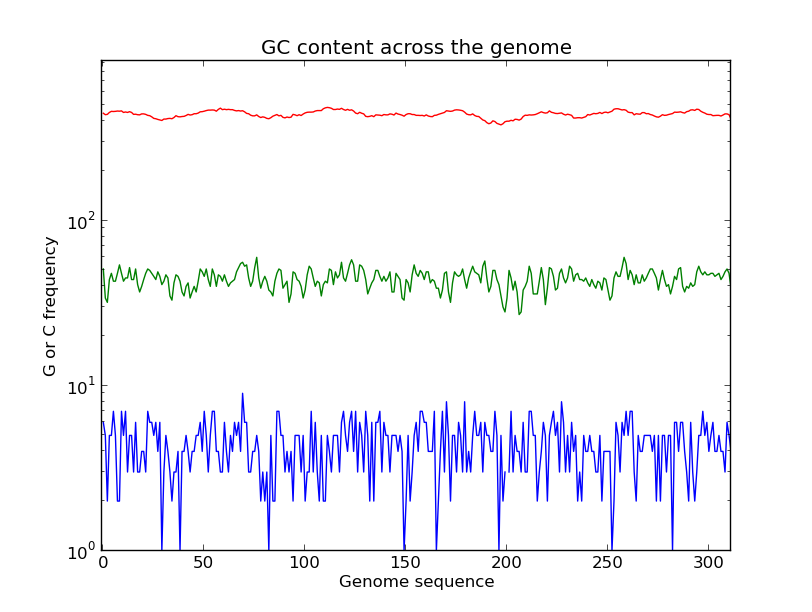
\includegraphics[scale=0.65]{3_log_all.png}
\caption{Red line - window size = 1000, green - window size 100, blue line - window size = 10.}
\label{log}
\end{center}
\end{figure}

\subsection{Chaos Game Representation}
Figure \ref{cgr} represents Chaos Game Representation for 3-mers and 4-mers.
\begin{figure}[h!]
\begin{center}
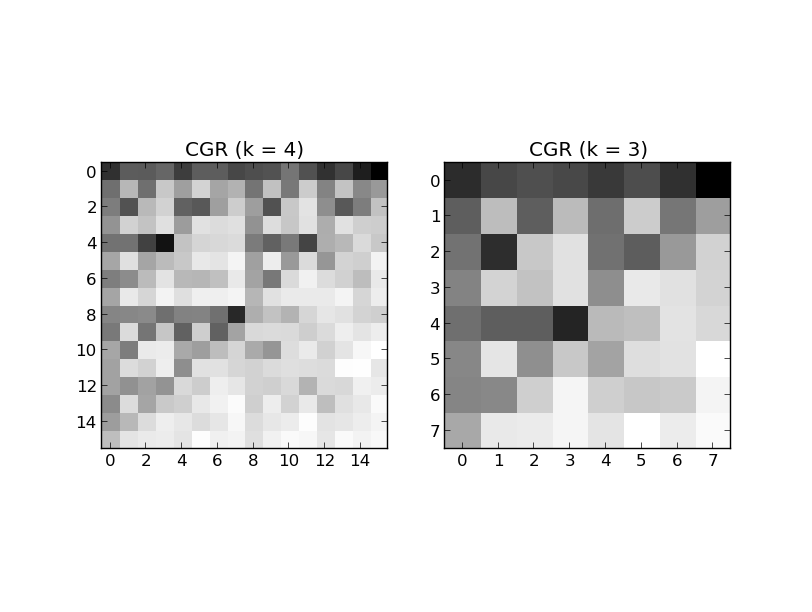
\includegraphics[scale=0.8]{4_cgr.png}
\caption{Chaos Game Representation for k = 4 and k = 3.}
\label{cgr}
\end{center}
\end{figure}

\section*{Honor Code}

% The following paragraph of your report should be included as is - do % not change it.

My answers to homework are my own work. I did not make solutions or code available to anyone else. I did not engage in any other activities that will dishonestly improve my results or dishonestly improve/hurt the results of others.

\end{document}